%==============================================================================
%  CHAPTER 15: Convergence Analysis
%  Part II: Optimization Theory
%==============================================================================
\documentclass[../../main.tex]{subfiles}

\begin{document}

\chapter{Convergence Analysis}
\label{ch:convergence-analysis}

Some optimization algorithms are provably 100x faster than others on the same problem. Convergence analysis tells you which algorithms will work---and how long they'll take---before you spend a single GPU hour. It's the difference between science and expensive guessing.

\begin{whycare}
Understanding convergence rates lets you debug slow training, choose hyperparameters intelligently, and predict compute requirements. When training runs cost thousands of dollars, being able to analyze convergence saves real money.
\end{whycare}

\begin{keyconcept}
Convergence analysis provides the mathematical framework for understanding when and how optimization algorithms find solutions. This chapter develops the theoretical foundations---Lipschitz continuity, strong convexity, and smoothness---that govern convergence rates for gradient descent and its variants. Understanding these concepts enables practitioners to select appropriate algorithms and hyperparameters for their specific optimization problems.
\end{keyconcept}

\begin{realworld}
\textbf{Why This Matters:} Understanding convergence rates helps you debug training and choose hyperparameters.

\textbf{Real Example:} Learning rate schedulers (cosine decay, warmup) are designed based on convergence theory.

\textbf{Scale:} Theoretical analysis predicted transformer scaling laws before they were empirically verified.
\end{realworld}

\begin{principle}
This chapter focuses on \textbf{what convergence results mean for practice}. Detailed proofs marked with $\star$ can be skipped on first reading; full proofs appear in Appendix~\ref{app:proofs}.
\end{principle}

\begin{keyconcept}
\textbf{Why This Matters in Modern ML:}
When training stalls or diverges, convergence theory provides the diagnostic framework. The condition number $\kappa$ explains why some problems train slowly---and why techniques like batch normalization and adaptive optimizers help by improving conditioning. Learning rate selection follows directly from smoothness bounds. Understanding why $O(1/\sqrt{\kappa})$ acceleration matters explains the ubiquity of momentum. These concepts transform hyperparameter tuning from trial-and-error into principled engineering.
\end{keyconcept}

\begin{intuition}[What to Expect]
This chapter is more theoretical than others. Here's how to navigate it:

\textbf{Essential concepts} (read carefully):
\begin{itemize}
    \item Convergence rates: What $O(1/t)$ vs $O(\rho^t)$ mean in practice
    \item Condition number $\kappa = L/\mu$: The single most important quantity for convergence speed
    \item The summary tables (Tables~\ref{tab:oracle-complexity} and~\ref{tab:convergence-summary})
\end{itemize}

\textbf{Can skip on first reading}:
\begin{itemize}
    \item Detailed proofs (marked with $\star$)---understand the theorem statements, return to proofs later
    \item Lower bounds and optimality (Section~\ref{sec:lower-bounds})---important for theory, less so for practice
\end{itemize}

\textbf{The payoff}: Understanding why ill-conditioning slows convergence explains why adaptive optimizers (Adam) often outperform vanilla SGD, and why learning rate selection matters so much.
\end{intuition}

\begin{prerequisites}
\textbf{Before reading this chapter, you should be comfortable with:}
\begin{itemize}
    \item Gradient descent and its variants (Chapters~\ref{ch:gradient-descent}, \ref{ch:advanced-optimizers})
    \item Convexity and strong convexity (Chapter~\ref{ch:convex-optimization})
    \item Big-O notation for algorithm analysis
\end{itemize}
\textbf{Review if needed:} Chapter~\ref{ch:convex-optimization} for convexity definitions, Chapter~\ref{ch:stochastic-optimization} for SGD analysis
\end{prerequisites}

%------------------------------------------------------------------------------
\section{Introduction}
\label{sec:conv-intro}

In previous chapters, we introduced momentum methods (Chapter~\ref{ch:gradient-descent}) and adaptive optimizers such as Adam and AdaGrad (Chapter~\ref{ch:advanced-optimizers}), and explored stochastic optimization fundamentals (Chapter~\ref{ch:stochastic-optimization}). A natural question arises: \textit{How fast do these algorithms converge, and under what conditions are they guaranteed to find a solution?}

Convergence analysis answers these questions by establishing mathematical relationships between problem properties (such as smoothness and convexity) and algorithm behavior (such as convergence rate and final accuracy). This analysis is not merely theoretical---it directly informs practical decisions about learning rate selection, algorithm choice, and computational budgeting.

\begin{intuition}
Think of optimization as navigating a landscape. The properties of the terrain---whether it has gentle slopes or steep cliffs, single valleys or multiple basins---determine how quickly and reliably you can reach the bottom. Convergence analysis quantifies these terrain properties mathematically.
\end{intuition}

%------------------------------------------------------------------------------
\section{Fundamental Concepts}
\label{sec:conv-fundamentals}

\subsection{Convergence Rates}

\begin{definition}{Convergence Rate}{conv-rate-def}
The \textbf{convergence rate}\index{convergence rate|textbf} of an optimization algorithm describes how quickly the distance to the optimum (or the suboptimality gap) decreases with the number of iterations $t$.

Common convergence rates include:
\begin{itemize}
    \item \textbf{Sublinear}\index{sublinear convergence}: $f(\vect{\theta}_t) - f(\vect{\theta}^*) = O(1/t^\alpha)$ for some $\alpha > 0$
    \item \textbf{Linear}\index{linear convergence|textbf}: $f(\vect{\theta}_t) - f(\vect{\theta}^*) = O(\rho^t)$ for some $\rho \in (0, 1)$
    \item \textbf{Superlinear}\index{superlinear convergence}: Faster than any geometric rate, e.g., $O(\rho^{t^2})$
    \item \textbf{Quadratic}\index{quadratic convergence}: $\norm{\vect{\theta}_{t+1} - \vect{\theta}^*} \leq C \norm{\vect{\theta}_t - \vect{\theta}^*}^2$
\end{itemize}
\end{definition}

\begin{important}
Despite the naming convention, ``linear convergence'' is actually exponentially fast in the number of iterations, since $\rho^t$ decreases exponentially. The term ``linear'' refers to the linear relationship $\log(f(\vect{\theta}_t) - f(\vect{\theta}^*)) \approx t \log \rho$. Sublinear convergence ($O(1/t)$) is polynomial, hence slower than linear.
\end{important}

\begin{aha}
\textbf{Memory trick:} ``Linear'' refers to the log-scale plot---$\log(\text{error})$ vs.\ iteration is a straight line. ``Sublinear'' curves away. If in doubt: linear = fast (exponential decay), sublinear = slow (polynomial decay).
\end{aha}

\begin{figure}[htbp]
\centering
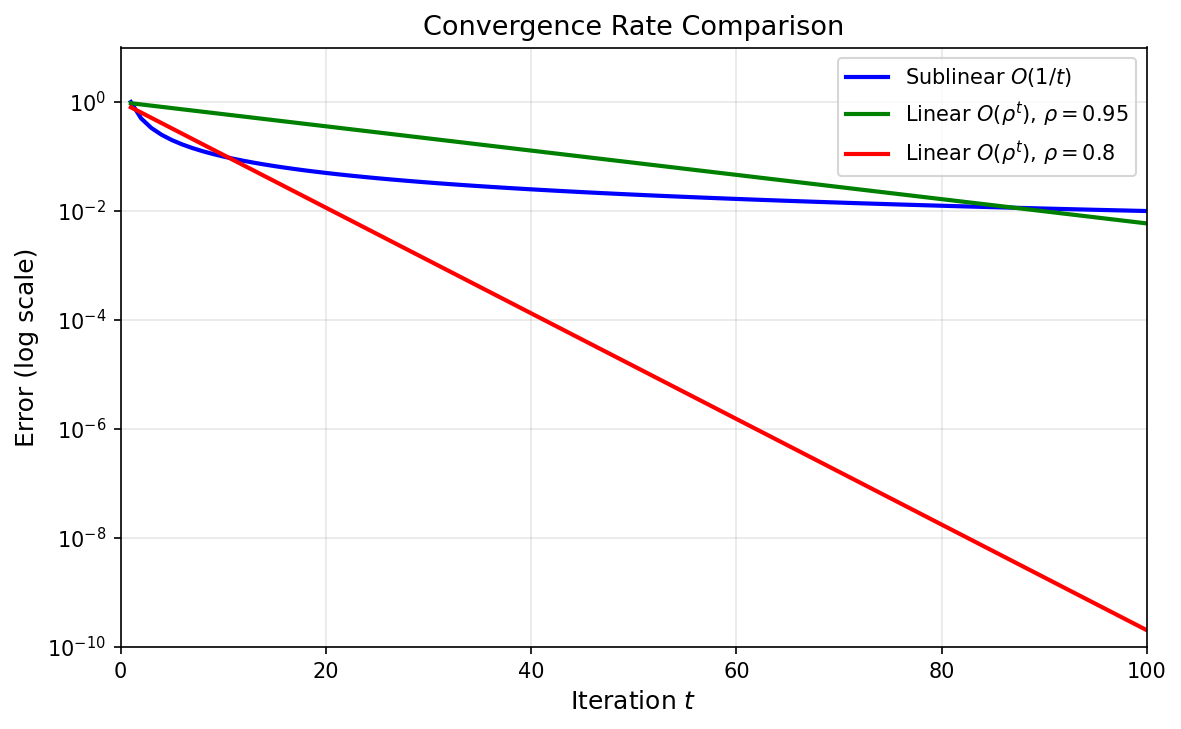
\includegraphics[width=0.8\textwidth]{../../images/diagrams/ch15/fig-convergence-rates.png}
\caption{Comparison of convergence rates on a semi-log scale. Sublinear $O(1/t)$ convergence (blue) decreases slowly. Linear convergence $O(\rho^t)$ with $\rho=0.95$ (green) and $\rho=0.8$ (red) shows exponential decay---the smaller $\rho$, the faster convergence.}
\label{fig:ch15-convergence-rates}
\end{figure}

\begin{example}{Comparing Convergence Rates}{conv-rate-comparison}
Consider reaching $\epsilon$-accuracy: $f(\vect{\theta}_t) - f(\vect{\theta}^*) \leq \epsilon$.

\begin{itemize}
    \item \textbf{$O(1/t)$ convergence}: Requires $t = O(1/\epsilon)$ iterations
    \item \textbf{$O(1/t^2)$ convergence}: Requires $t = O(1/\sqrt{\epsilon})$ iterations
    \item \textbf{Linear convergence} with $\rho = 0.99$: Requires $t = O(\log(1/\epsilon))$ iterations
\end{itemize}

For $\epsilon = 10^{-6}$: sublinear needs $10^6$ iterations, accelerated sublinear needs $10^3$ iterations, and linear convergence needs only about $1380$ iterations.
\end{example}

\subsection{Lipschitz Continuity}

\begin{definition}{Lipschitz Continuous Function}{lipschitz-def}
A function $f: \R^n \to \R$ is \textbf{$L$-Lipschitz continuous}\index{Lipschitz continuity|textbf}\index{Lipschitz constant} if there exists a constant $L \geq 0$ such that for all $\vect{x}, \vect{y} \in \R^n$:
\[
    |f(\vect{x}) - f(\vect{y})| \leq L \norm{\vect{x} - \vect{y}}
\]
The smallest such $L$ is called the \textbf{Lipschitz constant} of $f$.
\end{definition}

\begin{intuition}
Lipschitz continuity bounds how fast a function can change. If $f$ is $L$-Lipschitz, then moving a unit distance in the input space changes the function value by at most $L$. This prevents the function from having vertical asymptotes or infinite slopes.
\end{intuition}

\begin{definition}{Lipschitz Continuous Gradient (Smoothness)}{lipschitz-grad-def}
A differentiable function $f: \R^n \to \R$ has an \textbf{$L$-Lipschitz continuous gradient}\index{Lipschitz gradient} if:
\[
    \norm{\grad f(\vect{x}) - \grad f(\vect{y})} \leq L \norm{\vect{x} - \vect{y}} \quad \forall \vect{x}, \vect{y}
\]
Such functions are equivalently called \textbf{$L$-smooth}\index{smoothness|textbf} or said to have \textbf{smoothness parameter $L$}. This is equivalent to saying the Hessian (when it exists) has bounded eigenvalues: $\norm{\mat{H}(\vect{x})} \leq L$ for all $\vect{x}$.

Smoothness quantifies how ``well-behaved'' the gradient is. A smooth function doesn't have abrupt changes in slope, which means gradient descent can safely take larger steps without overshooting. The smoothness constant $L$ directly determines the maximum safe learning rate: $\eta \leq 1/L$.
\end{definition}

\begin{theorem}{Quadratic Upper Bound}{descent-lemma}
If $f$ has $L$-Lipschitz continuous gradients, then for all $\vect{x}, \vect{y}$:
\[
    f(\vect{y}) \leq f(\vect{x}) + \grad f(\vect{x})\trans (\vect{y} - \vect{x}) + \frac{L}{2}\norm{\vect{y} - \vect{x}}^2
\]
This is known as the \textbf{descent lemma}\index{descent lemma|textbf} and is fundamental to convergence proofs.
\end{theorem}

\begin{proof}[$\star$ Optional---can skip]
\textbf{Sketch:} Integrate the gradient along the line from $\vect{x}$ to $\vect{y}$, then bound the deviation using Lipschitz continuity. For the full proof, see Appendix~\ref{app:proofs}.
\end{proof}

%------------------------------------------------------------------------------
\subsection{Smoothness Implications}
\label{sec:smoothness}

\begin{lemma}{Smoothness Implications}{smoothness-implications}
For an $L$-smooth function $f$:
\begin{enumerate}
    \item \textbf{Quadratic upper bound}\index{quadratic upper bound}:
    \[
        f(\vect{y}) \leq f(\vect{x}) + \grad f(\vect{x})\trans (\vect{y} - \vect{x}) + \frac{L}{2}\norm{\vect{y} - \vect{x}}^2
    \]

    \item \textbf{Co-coercivity}\index{co-coercivity} (for convex $f$):
    \[
        (\grad f(\vect{x}) - \grad f(\vect{y}))\trans (\vect{x} - \vect{y}) \geq \frac{1}{L}\norm{\grad f(\vect{x}) - \grad f(\vect{y})}^2
    \]

    \item \textbf{Gradient bounds}\index{gradient bounds}:
    \[
        f(\vect{x}) - f(\vect{y}) \geq \grad f(\vect{y})\trans (\vect{x} - \vect{y}) + \frac{1}{2L}\norm{\grad f(\vect{x}) - \grad f(\vect{y})}^2
    \]
\end{enumerate}
\end{lemma}

\begin{figure}[htbp]
\centering
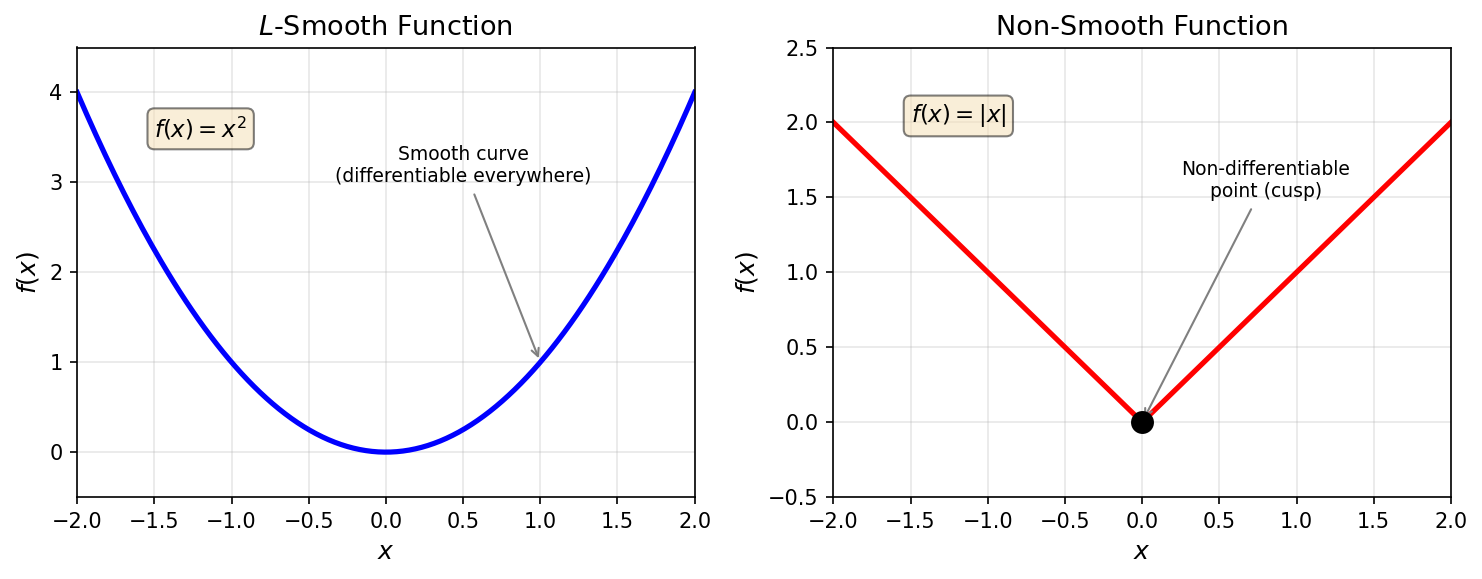
\includegraphics[width=0.8\textwidth]{../../images/diagrams/ch15/fig-smoothness.png}
\caption{Smoothness illustrated: an $L$-smooth function (solid blue) is bounded above by a quadratic with curvature $L$ (dashed) at every point. The gradient cannot change faster than $L$ times the distance moved, ensuring predictable optimization behavior.}
\label{fig:ch15-smoothness}
\end{figure}

%------------------------------------------------------------------------------
\section{Strong Convexity}
\label{sec:strong-convexity}

\begin{definition}{Strong Convexity}{strong-convex-def}
A function $f: \R^n \to \R$ is \textbf{$\mu$-strongly convex}\index{strong convexity|textbf} (with $\mu > 0$) if for all $\vect{x}, \vect{y}$:
\[
    f(\vect{y}) \geq f(\vect{x}) + \grad f(\vect{x})\trans (\vect{y} - \vect{x}) + \frac{\mu}{2}\norm{\vect{y} - \vect{x}}^2
\]
Equivalently, $f(\vect{x}) - \frac{\mu}{2}\norm{\vect{x}}^2$ is convex.
\end{definition}

\begin{intuition}
Strong convexity means the function curves upward at least as fast as a quadratic with curvature $\mu$. This guarantees a unique global minimum and prevents the function from having flat regions where gradient descent would stall. The stronger the convexity (larger $\mu$), the faster gradient descent converges.
\end{intuition}

\begin{theorem}{Strong Convexity Characterizations}{strong-convex-chars}
For a twice-differentiable function $f$, the following are equivalent:
\begin{enumerate}
    \item $f$ is $\mu$-strongly convex
    \item $\mat{H}(\vect{x}) \succeq \mu \mat{I}$ for all $\vect{x}$ (minimum eigenvalue $\geq \mu$)
    \item $(\grad f(\vect{x}) - \grad f(\vect{y}))\trans (\vect{x} - \vect{y}) \geq \mu \norm{\vect{x} - \vect{y}}^2$
    \item $f(\vect{y}) \geq f(\vect{x}) + \grad f(\vect{x})\trans (\vect{y} - \vect{x}) + \frac{\mu}{2}\norm{\vect{y} - \vect{x}}^2$
\end{enumerate}
\end{theorem}

\begin{definition}{Condition Number}{ch15-condition-number-def}
For a $\mu$-strongly convex and $L$-smooth function, the \textbf{condition number}\index{condition number|textbf} is:
\[
    \kappa = \frac{L}{\mu}
\]
For quadratic functions $f(\vect{x}) = \frac{1}{2}\vect{x}\trans \mat{A} \vect{x}$, this equals the ratio of the largest to smallest eigenvalue of $\mat{A}$: $\kappa = \lambda_{\max}/\lambda_{\min}$.
\end{definition}

\begin{important}
The condition number $\kappa$ is the single most important quantity governing convergence speed:
\begin{itemize}
    \item $\kappa = 1$: Perfect conditioning (isotropic curvature), fastest convergence
    \item $\kappa \gg 1$: Ill-conditioned\index{ill-conditioning} problem, slow convergence
    \item $\kappa \to \infty$: The function approaches non-strong convexity
\end{itemize}
Many optimization challenges in machine learning stem from ill-conditioned loss landscapes~\cite{goodfellow2016deep}.

Deep networks without batch normalization can have condition numbers in the thousands or higher. Adding batch normalization typically reduces the effective condition number substantially---potentially by one or two orders of magnitude---which partly explains why BatchNorm enables training much deeper networks.
\end{important}

\begin{aha}
The condition number $\kappa$ explains why some problems train 1000x slower than others. If your loss landscape is ``elongated'' (high $\kappa$), gradient descent zigzags back and forth. Techniques like Adam, batch normalization, and proper initialization all work by reducing the effective condition number.
\end{aha}

\begin{intuition}
Think of condition number as the aspect ratio of a room you're trying to cross. With $\kappa = 1$ (a square room), you can walk straight to your destination. With $\kappa = 100$ (a long, narrow hallway), you keep bouncing off the walls, making slow zigzag progress. Preconditioning (like batch normalization) reshapes the hallway into a more square room.
\end{intuition}

\begin{figure}[htbp]
\centering
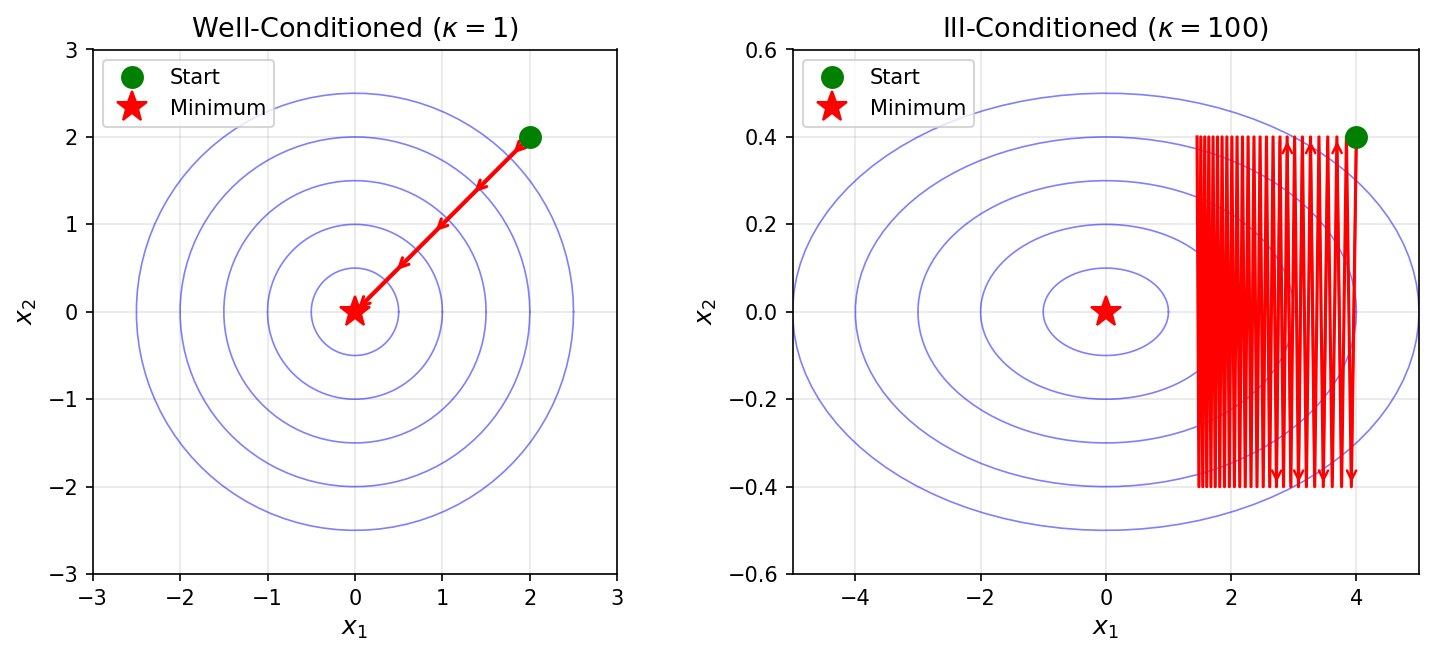
\includegraphics[width=0.8\textwidth]{../../images/diagrams/ch15/fig-condition-number.png}
\caption{Effect of condition number on gradient descent trajectories. Left: well-conditioned problem ($\kappa \approx 1$) with circular contours allows direct descent. Right: ill-conditioned problem ($\kappa \gg 1$) with elongated contours causes zigzag behavior, dramatically slowing convergence.}
\label{fig:ch15-condition-number}
\end{figure}

\begin{checkpoint}
For a quadratic function with Hessian eigenvalues 100 and 1, what is the condition number? How many iterations would gradient descent need to reduce the error by a factor of 100?
\end{checkpoint}

\begin{commonmistakes}
\begin{itemize}
    \item \textbf{Mistake:} Interpreting ``linear convergence'' as slow (linear in iterations)

    \textbf{Why it's wrong:} In optimization, ``linear convergence'' means the error decreases by a constant factor each iteration: $\epsilon_t = \rho^t \epsilon_0$. This is actually \emph{exponential} decay---very fast! The term ``linear'' refers to the linear relationship when you plot $\log(\epsilon_t)$ vs $t$.

    \textbf{Correct understanding:} Linear convergence $O(\rho^t)$ is fast (exponential decay). Sublinear $O(1/t)$ is slow (polynomial decay). ``Linear'' is named for the log-scale plot, not the iteration count.
\end{itemize}
\end{commonmistakes}

%------------------------------------------------------------------------------
\section{Convergence of Gradient Descent}
\label{sec:gd-convergence}

\subsection{Convergence for Smooth Convex Functions}

\begin{theorem}{GD Convergence: Smooth Convex}{gd-smooth-convex}
Let $f$ be convex with $L$-Lipschitz continuous gradients. Gradient descent with step size $\eta = 1/L$ satisfies:
\[
    f(\vect{\theta}_t) - f(\vect{\theta}^*) \leq \frac{L \norm{\vect{\theta}_0 - \vect{\theta}^*}^2}{2t}
\]
This is an $O(1/t)$ convergence rate.
\end{theorem}

\begin{proof}[$\star$ Optional---can skip]
\textbf{Sketch:} Apply the descent lemma to show each step decreases $f$ by at least $\frac{1}{2L}\norm{\grad f}^2$. Combined with convexity, this gives a telescoping sum that yields the $O(1/t)$ rate. For the full proof, see Appendix~\ref{app:proofs}.
\end{proof}

\subsection{Convergence for Strongly Convex Functions}

\begin{theorem}{GD Convergence: Strongly Convex and Smooth}{gd-strong-convex-smooth}
Let $f$ be $\mu$-strongly convex with $L$-Lipschitz continuous gradients. Gradient descent with step size $\eta = 1/L$ achieves:
\[
    f(\vect{\theta}_t) - f(\vect{\theta}^*) \leq \left(1 - \frac{\mu}{L}\right)^t [f(\vect{\theta}_0) - f(\vect{\theta}^*)]
\]
Equivalently:
\[
    \norm{\vect{\theta}_t - \vect{\theta}^*}^2 \leq \left(1 - \frac{\mu}{L}\right)^t \norm{\vect{\theta}_0 - \vect{\theta}^*}^2
\]
This is \textbf{linear convergence} with rate $\rho = 1 - 1/\kappa$.
\end{theorem}

\begin{proof}[$\star$ Optional---can skip]
\textbf{Sketch:} Strong convexity provides a lower bound $\norm{\grad f}^2 \geq 2\mu(f - f^*)$. Combined with the descent lemma's guarantee of per-step progress, we get $\delta_{t+1} \leq (1 - \mu/L)\delta_t$, which yields linear convergence by induction. For the full proof, see Appendix~\ref{app:proofs}.
\end{proof}

\begin{keyconcept}
The convergence rate depends critically on the condition number $\kappa = L/\mu$:
\begin{itemize}
    \item \textbf{Well-conditioned} ($\kappa \approx 1$): Rapid convergence, $\rho \approx 0$
    \item \textbf{Moderately conditioned} ($\kappa = 100$): $\rho = 0.99$, needs $\sim 460$ iterations for $\epsilon = 10^{-2}$
    \item \textbf{Ill-conditioned} ($\kappa = 10^6$): $\rho \approx 1$, extremely slow convergence
\end{itemize}
\end{keyconcept}

%------------------------------------------------------------------------------
\section{Convergence of Stochastic Gradient Descent}
\label{sec:sgd-convergence-ch15}

SGD introduces variance due to random sampling, which fundamentally changes the convergence behavior.

\begin{definition}{SGD Assumptions}{sgd-assumptions}
For SGD convergence analysis, we typically assume:
\begin{enumerate}
    \item \textbf{Unbiased gradients}: $\E[\vect{g}_t | \vect{\theta}_t] = \grad f(\vect{\theta}_t)$
    \item \textbf{Bounded variance}: $\E[\norm{\vect{g}_t - \grad f(\vect{\theta}_t)}^2] \leq \sigma^2$
    \item \textbf{Smoothness}: $f$ has $L$-Lipschitz gradients
\end{enumerate}
\end{definition}

\subsection{SGD for Convex Functions}

\begin{theorem}{SGD Convergence: Convex}{sgd-convex}
For convex $f$ with $L$-smooth gradients and bounded variance $\sigma^2$, SGD with step size $\eta_t = \eta_0/\sqrt{t}$ achieves:
\[
    \E[f(\bar{\vect{\theta}}_T)] - f(\vect{\theta}^*) = O\left(\frac{\norm{\vect{\theta}_0 - \vect{\theta}^*}^2 + \sigma^2}{\sqrt{T}}\right)
\]
where $\bar{\vect{\theta}}_T = \frac{1}{T}\sum_{t=1}^T \vect{\theta}_t$ is the average iterate.
\end{theorem}

\begin{intuition}
SGD's convergence is slower than full GD due to gradient variance. The $O(1/\sqrt{T})$ rate reflects the fundamental trade-off: we gain computational efficiency by using stochastic gradients but pay with slower convergence. The variance term $\sigma^2$ quantifies this cost.
\end{intuition}

\subsection{SGD for Strongly Convex Functions}

\begin{theorem}{SGD Convergence: Strongly Convex}{sgd-strong-convex}
For $\mu$-strongly convex $f$ with bounded variance $\sigma^2$, SGD with decreasing step size $\eta_t = 2/(\mu(t+1))$ achieves:
\[
    \E[f(\vect{\theta}_T)] - f(\vect{\theta}^*) = O\left(\frac{\sigma^2}{\mu T}\right)
\]
This is an $O(1/T)$ rate, which improves upon the non-strongly convex case.
\end{theorem}

\begin{theorem}{SGD with Constant Step Size}{sgd-constant-lr}
For $\mu$-strongly convex and $L$-smooth $f$, SGD with constant step size $\eta < 1/L$ converges to a neighborhood of the optimum:
\[
    \E[\norm{\vect{\theta}_t - \vect{\theta}^*}^2] \leq (1 - \mu\eta)^t \norm{\vect{\theta}_0 - \vect{\theta}^*}^2 + \frac{\eta \sigma^2}{\mu}
\]
The algorithm converges linearly to an $O(\eta\sigma^2/\mu)$ ball around the optimum but cannot reach the optimum exactly.
\end{theorem}

\begin{important}
\textbf{The SGD Trade-off}: With constant step size, SGD oscillates in a ball around the optimum, never converging exactly. Decreasing step sizes allow convergence to the optimum but slow down learning. This motivates:
\begin{itemize}
    \item Learning rate schedules that decay over time
    \item Variance reduction techniques\index{variance reduction} (SVRG\index{SVRG}, SAGA\index{SAGA})
    \item Mini-batching\index{mini-batch!variance reduction} to reduce variance
\end{itemize}
\end{important}

\begin{figure}[htbp]
\centering
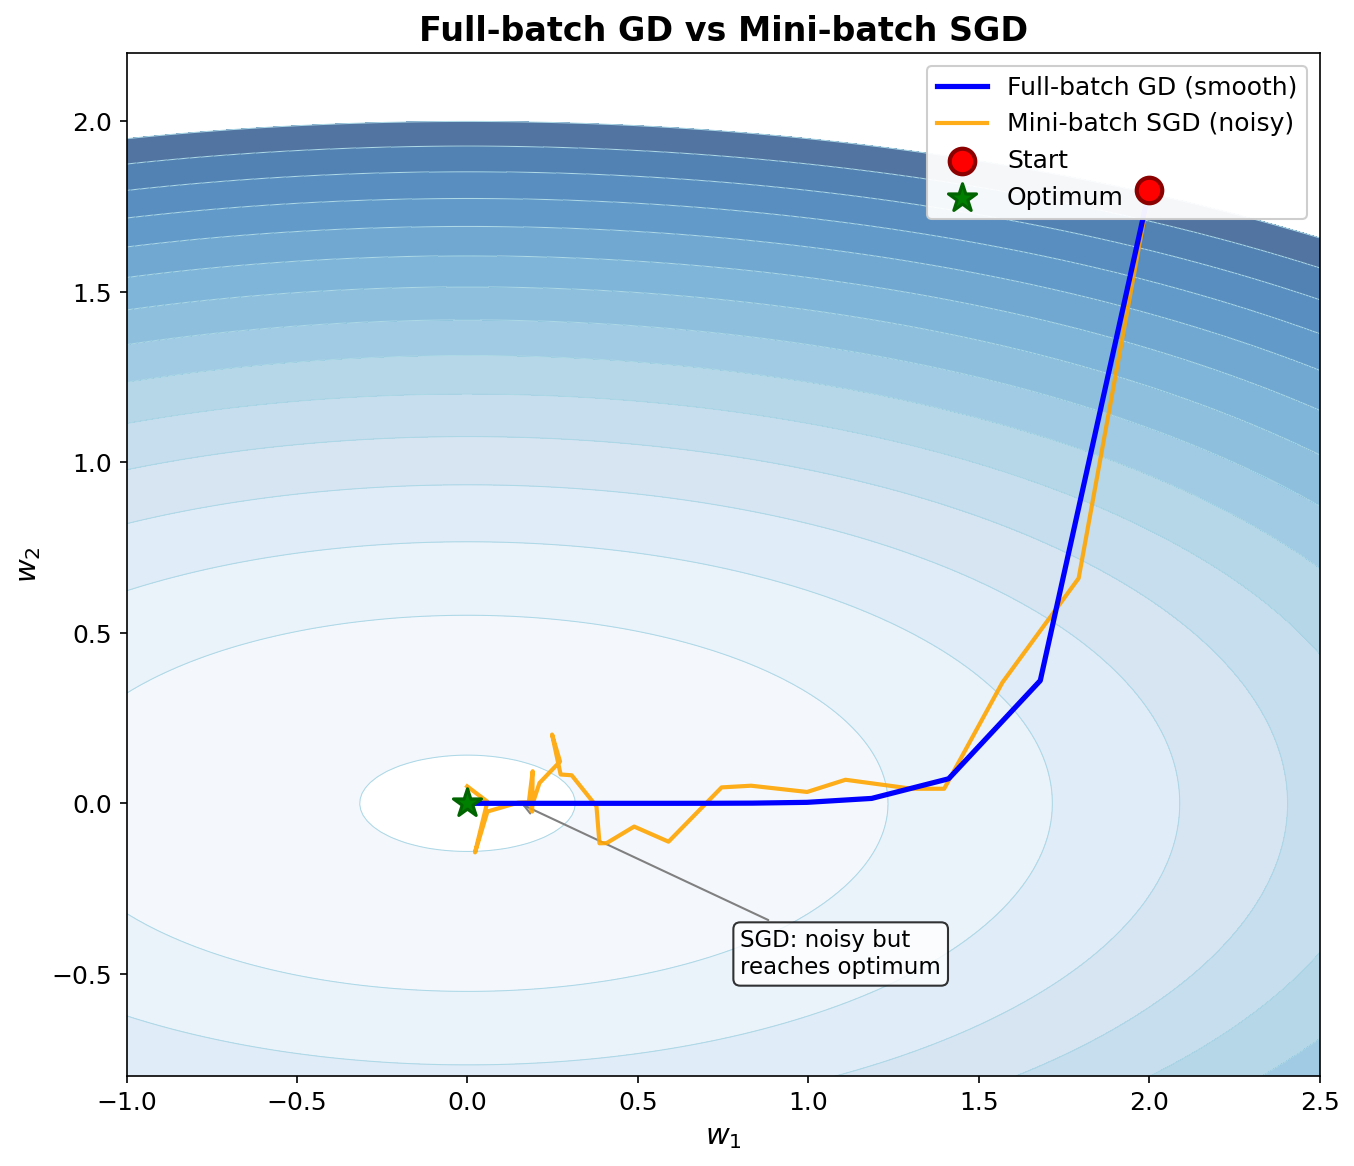
\includegraphics[width=0.8\textwidth]{../../images/diagrams/ch15/fig-sgd-vs-gd.png}
\caption{Comparison of gradient descent (GD) and stochastic gradient descent (SGD) convergence. GD (blue) follows a smooth path to the optimum. SGD (orange) exhibits noisy oscillations due to gradient variance but often converges faster in wall-clock time due to cheaper per-iteration cost.}
\label{fig:ch15-sgd-vs-gd}
\end{figure}

\subsection{Mini-Batch SGD}

\begin{theorem}{Mini-Batch Variance Reduction}{minibatch-variance}
Using mini-batches of size $B$ reduces the gradient variance:
\[
    \Var\left[\frac{1}{B}\sum_{i \in \mathcal{B}} \grad L_i(\vect{\theta})\right] = \frac{\sigma^2}{B}
\]
where $\sigma^2$ is the single-sample variance. This leads to tighter convergence:
\[
    \E[\norm{\vect{\theta}_t - \vect{\theta}^*}^2] \leq (1 - \mu\eta)^t \norm{\vect{\theta}_0 - \vect{\theta}^*}^2 + \frac{\eta \sigma^2}{\mu B}
\]
\end{theorem}

%------------------------------------------------------------------------------
\section{Accelerated Methods}
\label{sec:acceleration}

\subsection{Nesterov's Accelerated Gradient}

\begin{theorem}{Nesterov Acceleration}{ch15-nesterov-rate}
\index{Nesterov acceleration|textbf}\index{accelerated gradient descent|see{Nesterov acceleration}}For convex $f$ with $L$-Lipschitz gradients, Nesterov's accelerated gradient descent achieves:
\[
    f(\vect{\theta}_t) - f(\vect{\theta}^*) \leq \frac{2L\norm{\vect{\theta}_0 - \vect{\theta}^*}^2}{(t+1)^2}
\]
This is an $O(1/t^2)$ rate, improving upon vanilla GD's $O(1/t)$.
\end{theorem}

\begin{definition}{Nesterov Accelerated Gradient}{nag-def}
Nesterov's method uses a momentum-like update with a ``look-ahead'' gradient:
\begin{align*}
    \vect{y}_t &= \vect{\theta}_t + \frac{t-1}{t+2}(\vect{\theta}_t - \vect{\theta}_{t-1}) \\
    \vect{\theta}_{t+1} &= \vect{y}_t - \eta \grad f(\vect{y}_t)
\end{align*}
The momentum coefficient $\gamma_t = (t-1)/(t+2)$ is carefully chosen to achieve optimal convergence.
\end{definition}

\begin{theorem}{Accelerated Strongly Convex Convergence}{accelerated-strong-convex}
For $\mu$-strongly convex and $L$-smooth functions, Nesterov's method achieves:
\[
    f(\vect{\theta}_t) - f(\vect{\theta}^*) \leq L\norm{\vect{\theta}_0 - \vect{\theta}^*}^2 \left(1 - \frac{1}{\sqrt{\kappa}}\right)^t
\]
The convergence rate improves from $1 - 1/\kappa$ (vanilla GD) to $1 - 1/\sqrt{\kappa}$, which is significant for ill-conditioned problems.
\end{theorem}

\begin{example}{Acceleration Benefit}{acceleration-example}
Consider a problem with condition number $\kappa = 10^4$:
\begin{itemize}
    \item \textbf{Vanilla GD}: Rate $\rho = 1 - 10^{-4} = 0.9999$. Needs $\sim 92,000$ iterations for $10^{-4}$ accuracy.
    \item \textbf{Nesterov}: Rate $\rho = 1 - 10^{-2} = 0.99$. Needs $\sim 920$ iterations for same accuracy.
\end{itemize}
Acceleration provides a 100x speedup for this ill-conditioned problem.

For a neural network with condition number $\kappa = 10,000$ (common for deep networks without batch normalization), vanilla gradient descent needs approximately $20,000$ iterations while Nesterov acceleration needs only $200$---potentially the difference between days and hours of training, or a 100$\times$ compute cost reduction.
\end{example}

\begin{figure}[htbp]
\centering
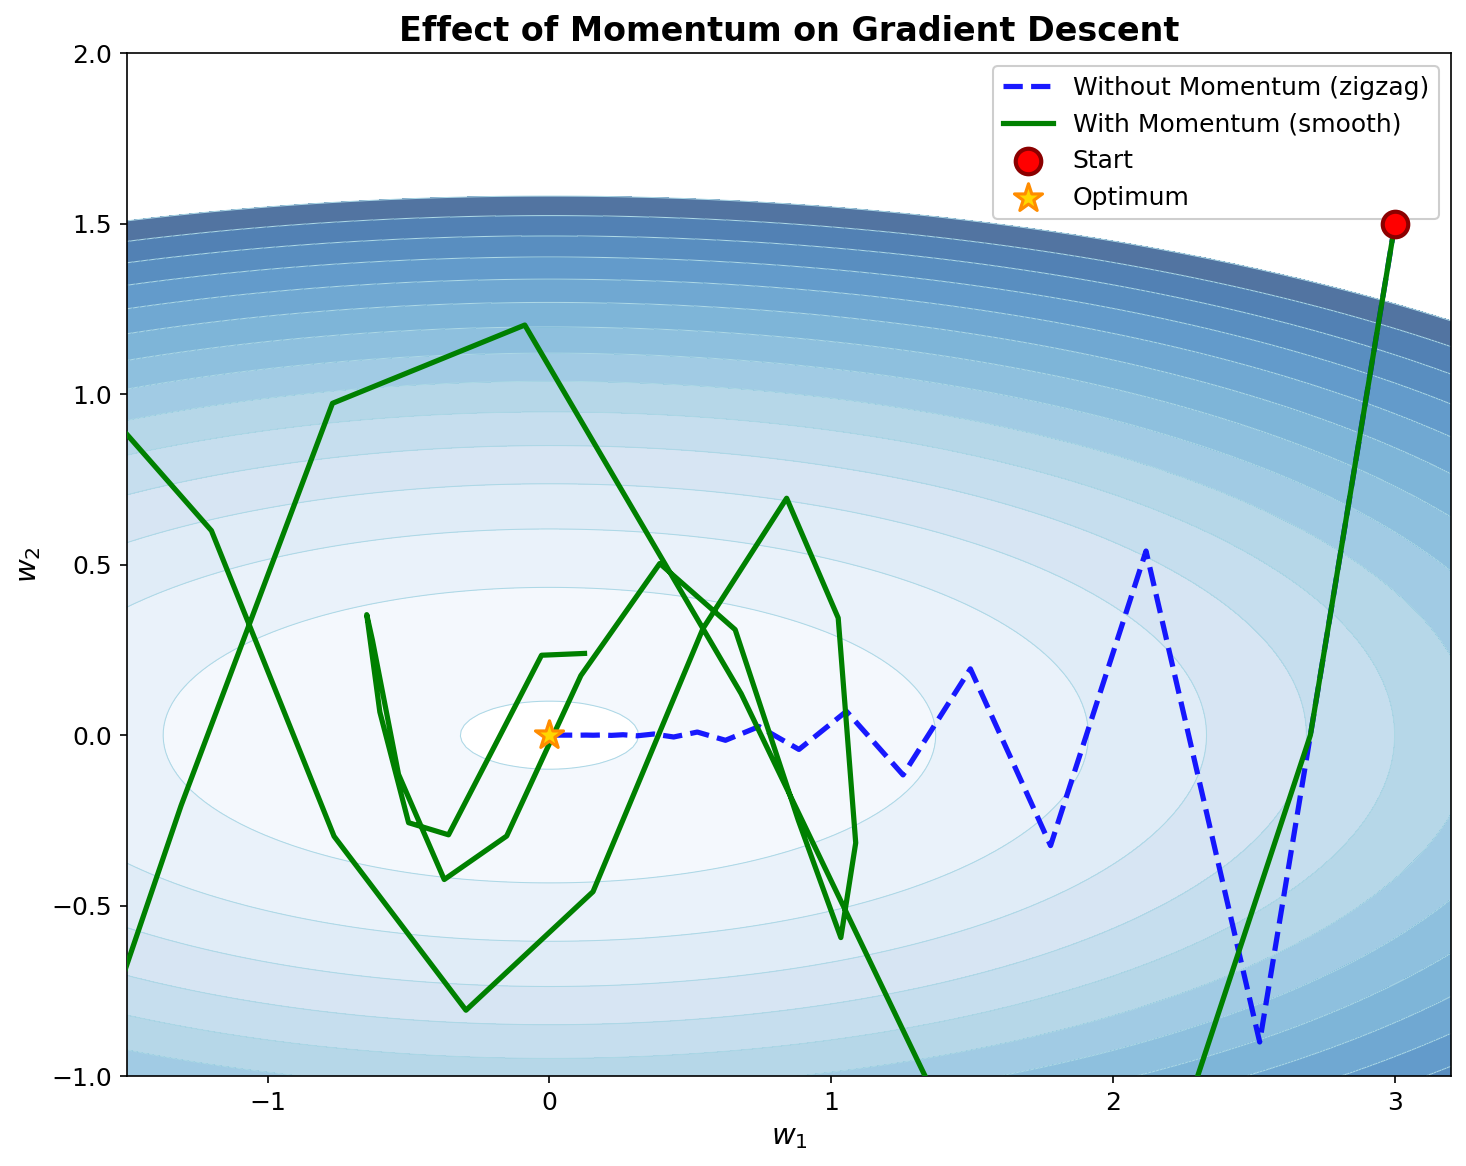
\includegraphics[width=0.8\textwidth]{../../images/diagrams/ch15/fig-momentum-effect.png}
\caption{Effect of momentum on optimization trajectories. Without momentum (blue), gradient descent oscillates across narrow valleys. With momentum (green), the optimizer accumulates velocity in consistent directions, damping oscillations and accelerating convergence along the dominant direction.}
\label{fig:ch15-momentum-effect}
\end{figure}

\begin{checkpoint}
What is the difference between $O(1/t)$ and $O(\rho^t)$ convergence? Which is faster and why?
\end{checkpoint}

\begin{checkpoint}
Why does momentum help optimization? Explain in terms of the condition number improvement from $O(1/\kappa)$ to $O(1/\sqrt{\kappa})$.
\end{checkpoint}

\subsection{Heavy Ball Method}

\begin{definition}{Polyak's Heavy Ball Method}{heavy-ball-def}
\index{heavy ball method|textbf}\index{Polyak momentum|see{heavy ball method}}The heavy ball method uses constant momentum:
\[
    \vect{\theta}_{t+1} = \vect{\theta}_t - \eta \grad f(\vect{\theta}_t) + \gamma(\vect{\theta}_t - \vect{\theta}_{t-1})
\]
where $\gamma \in [0, 1)$ is the momentum coefficient. With optimal parameters $\eta = 4/({\sqrt{L} + \sqrt{\mu}})^2$ and $\gamma = ((\sqrt{\kappa}-1)/(\sqrt{\kappa}+1))^2$ (where $L$ is the smoothness constant), it achieves the same rate as Nesterov's method for quadratic functions.
\end{definition}

\begin{important}
\textbf{Nesterov vs. Heavy Ball}:
\begin{itemize}
    \item Heavy Ball is optimal for quadratics but may not converge for general convex functions
    \item Nesterov's method is universally optimal for smooth convex functions
    \item In practice, both are often used with fixed momentum (e.g., 0.9) rather than optimal theoretical values
\end{itemize}
\end{important}

%------------------------------------------------------------------------------
\section{Lower Bounds and Optimality}
\label{sec:lower-bounds}

Are the convergence rates we've established the best possible? Lower bound theory answers this question.

\begin{theorem}{Lower Bound: Smooth Convex}{lower-bound-convex}
\index{lower bound!smooth convex}For the class of convex functions with $L$-Lipschitz gradients, any first-order method\index{first-order method} that uses only gradient information must satisfy:
\[
    f(\vect{\theta}_t) - f(\vect{\theta}^*) \geq \Omega\left(\frac{L\norm{\vect{\theta}_0 - \vect{\theta}^*}^2}{t^2}\right)
\]
for some ``hard'' function in this class.
\end{theorem}

\begin{theorem}{Lower Bound: Strongly Convex}{lower-bound-strong-convex}
For $\mu$-strongly convex functions with $L$-smooth gradients, any first-order method satisfies:
\[
    \norm{\vect{\theta}_t - \vect{\theta}^*}^2 \geq \Omega\left(\left(1 - \frac{1}{\sqrt{\kappa}}\right)^{2t}\right) \norm{\vect{\theta}_0 - \vect{\theta}^*}^2
\]
\end{theorem}

\begin{keyconcept}
\textbf{Optimality of Accelerated Methods}:
\begin{itemize}
    \item Nesterov's $O(1/t^2)$ rate matches the lower bound for smooth convex functions
    \item Nesterov's $O((1-1/\sqrt{\kappa})^t)$ rate matches the lower bound for strongly convex
    \item These methods are \textbf{optimal} among first-order methods
    \item Vanilla GD is suboptimal---its $O(1/t)$ or $O((1-1/\kappa)^t)$ rates have gaps from the lower bounds
\end{itemize}
\end{keyconcept}

\subsection{Oracle Complexity}

\begin{definition}{Oracle Complexity}{oracle-complexity}
The \textbf{oracle complexity}\index{oracle complexity|textbf} of an optimization problem is the minimum number of gradient evaluations (oracle calls) required to find an $\epsilon$-accurate solution. Here $D = \norm{\vect{\theta}_0 - \vect{\theta}^*}$.
\end{definition}

\begin{table}[htbp]
\centering
\caption{Oracle complexity for different problem classes.}
\label{tab:oracle-complexity}
\begin{tabular}{@{}lcc@{}}
\toprule
\textbf{Problem Class} & \textbf{Vanilla GD} & \textbf{Accelerated GD} \\
\midrule
$L$-smooth convex & $O(L D^2/\epsilon)$ & $O(\sqrt{L D^2/\epsilon})$ \\
$\mu$-strongly convex, $L$-smooth & $O(\kappa \log(1/\epsilon))$ & $O(\sqrt{\kappa} \log(1/\epsilon))$ \\
\bottomrule
\end{tabular}
\end{table}

%------------------------------------------------------------------------------
\section{Non-Convex Convergence}
\label{sec:nonconvex-convergence}

Deep learning involves non-convex optimization. What can we say about convergence?

\begin{theorem}{GD for Smooth Non-Convex Functions}{gd-nonconvex}
For a (possibly non-convex) function $f$ with $L$-Lipschitz gradients, gradient descent with $\eta = 1/L$ satisfies:
\[
    \min_{0 \leq t \leq T-1} \norm{\grad f(\vect{\theta}_t)}^2 \leq \frac{2L[f(\vect{\theta}_0) - f^*]}{T}
\]
where $f^* = \inf_{\vect{\theta}} f(\vect{\theta})$.
\end{theorem}

\begin{intuition}
For non-convex functions, we cannot guarantee convergence to a global minimum. Instead, we prove convergence to a \textbf{stationary point}\index{stationary point|textbf} where $\grad f(\vect{\theta}) = \mathbf{0}$. The theorem says gradient descent finds a point with small gradient in $O(1/\epsilon^2)$ iterations to reach $\norm{\grad f}^2 \leq \epsilon$.
\end{intuition}

\begin{theorem}{SGD for Non-Convex Functions}{sgd-nonconvex}
For non-convex $f$ with $L$-smooth gradients and stochastic gradients with bounded variance $\sigma^2$, SGD with $\eta_t = 1/(L\sqrt{T})$ satisfies:
\[
    \E\left[\min_{t \leq T} \norm{\grad f(\vect{\theta}_t)}^2\right] = O\left(\frac{f(\vect{\theta}_0) - f^* + \sigma^2}{\sqrt{T}}\right)
\]
\end{theorem}

\begin{important}
\textbf{Non-Convex Challenges}:
\begin{itemize}
    \item Stationary points may be saddle points\index{saddle point}, not local minima
    \item Convergence guarantees are to approximate stationary points, not optima
    \item The loss landscape of neural networks has many local minima, but empirically they often have similar loss values
    \item SGD's noise helps escape saddle points, partially explaining its success in deep learning
\end{itemize}
\end{important}

%------------------------------------------------------------------------------
\section{Convergence Rate Summary}
\label{sec:rate-summary}

\begin{table}[htbp]
\centering
\caption{Summary of convergence rates for different algorithms and problem classes.}
\label{tab:convergence-summary}
\begin{tabular}{@{}llll@{}}
\toprule
\textbf{Algorithm} & \textbf{Convex} & \textbf{Strongly Convex} & \textbf{Non-Convex} \\
\midrule
GD & $O(1/t)$ & $O((1-1/\kappa)^t)$ & $O(1/t)$ to stationary \\
Accelerated GD & $O(1/t^2)$ & $O((1-1/\sqrt{\kappa})^t)$ & -- \\
SGD (decreasing $\eta$) & $O(1/\sqrt{t})$ & $O(1/t)$ & $O(1/\sqrt{t})$ \\
SGD (constant $\eta$) & -- & $O(\eta\sigma^2)$ ball & -- \\
\bottomrule
\end{tabular}
\end{table}

%------------------------------------------------------------------------------
\section{Practical Implications}
\label{sec:practical-implications}

\subsection{Learning Rate Selection}

\begin{principle}
From convergence theory, the maximum stable learning rate is $\eta = 1/L$ (or $2/L$ for some analyses). In practice:
\begin{itemize}
    \item Estimate $L$ by computing gradient differences: $L \approx \norm{\grad f(\vect{x}) - \grad f(\vect{y})}/\norm{\vect{x} - \vect{y}}$
    \item Use learning rate schedules that start large and decay
    \item Adaptive methods (Adam) implicitly estimate and adapt to local smoothness
\end{itemize}
\end{principle}

\begin{figure}[htbp]
\centering
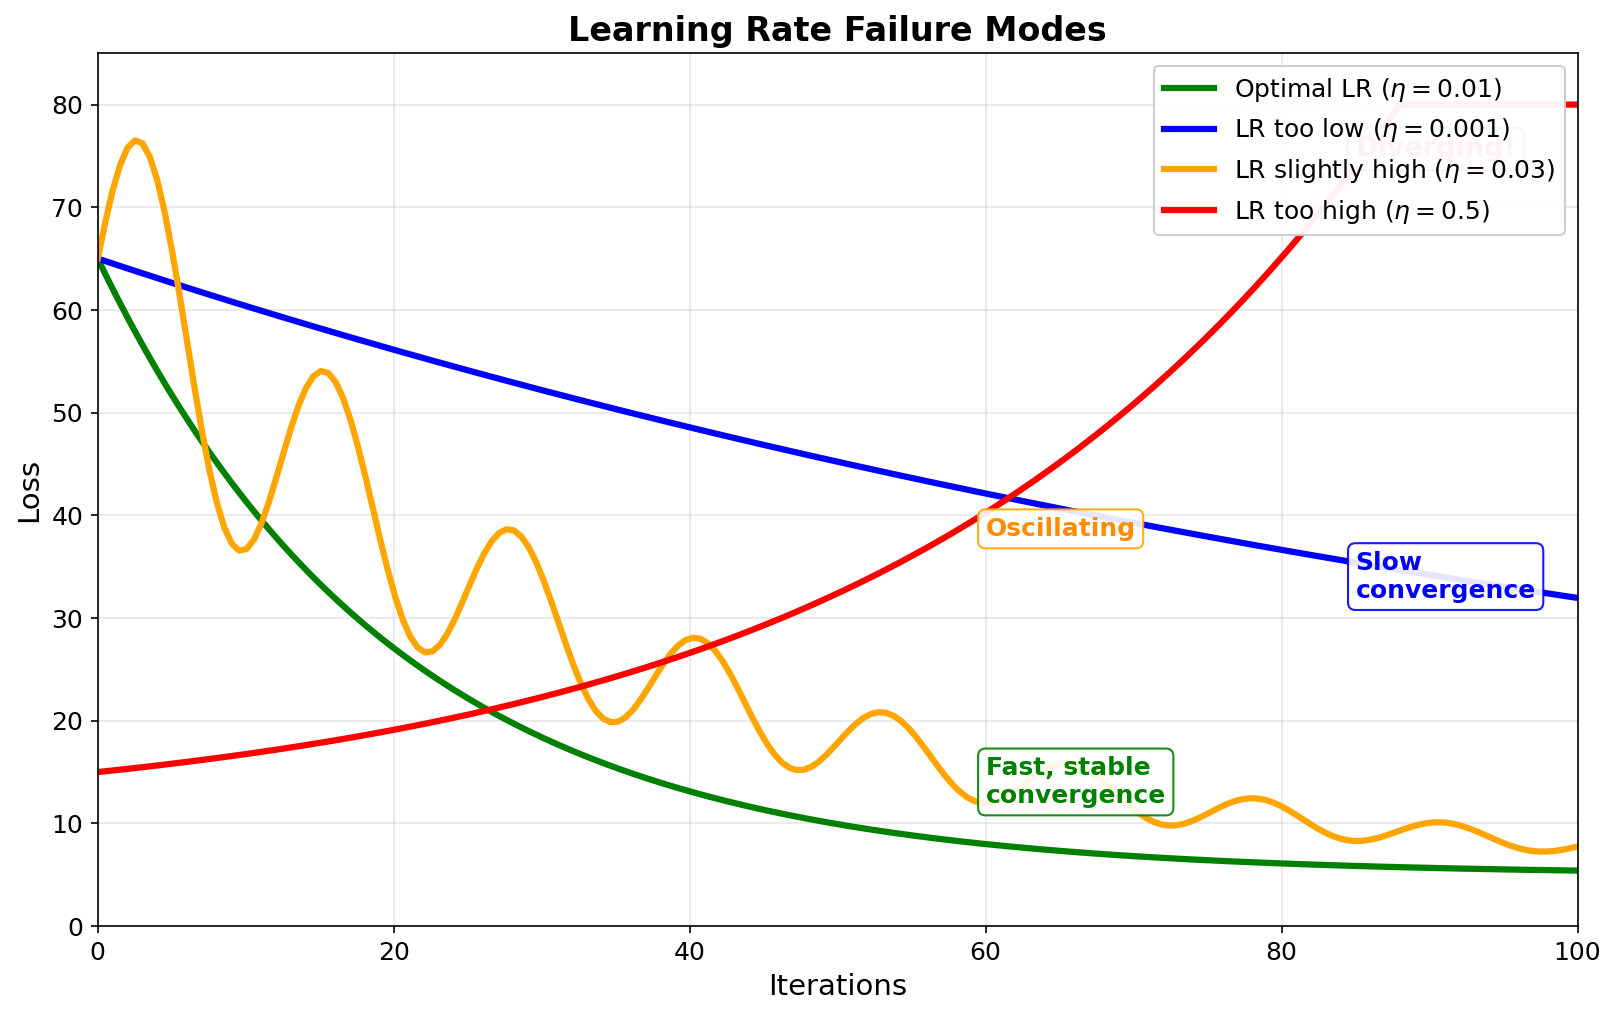
\includegraphics[width=0.8\textwidth]{../../images/diagrams/ch15/fig-lr-failure-modes.png}
\caption{Learning rate failure modes. Four scenarios are shown: optimal LR (green) converges smoothly and quickly; LR too low (blue) converges but extremely slowly; LR slightly high (orange) oscillates but eventually converges; LR too high (red) diverges. The smoothness constant $L$ determines the boundary between stable and unstable regimes.}
\label{fig:ch15-lr-failure-modes}
\end{figure}

\subsection{Batch Size Selection}

\begin{principle}[title=Linear Scaling Rule]
\index{linear scaling rule|textbf}\textbf{(Empirical Heuristic)} For SGD with mini-batch size $B$, if learning rate $\eta$ works well for $B = 1$, then learning rate $\eta \cdot B$ approximately maintains similar convergence behavior. This guideline (Goyal et al., 2017) is widely used but is not a theorem---it requires warmup and breaks down for very large batches.
\end{principle}

\begin{intuition}
Larger batches reduce variance by factor $B$, allowing proportionally larger learning rates. However, this relationship breaks down for very large batches due to the noise floor in the loss function and generalization considerations.
\end{intuition}

\subsection{Warmup and Schedules}

\begin{keyconcept}
Convergence theory suggests several practical strategies:
\begin{enumerate}
    \item \textbf{Learning rate warmup}\index{learning rate warmup}: Start with small $\eta$ to stabilize gradients, then increase
    \item \textbf{Decay schedules}\index{learning rate schedule}: Reduce $\eta$ to shrink SGD's convergence ball
    \item \textbf{Cosine annealing}\index{cosine annealing}: Smooth decay that approximates optimal decreasing schedule
    \item \textbf{Restarts}\index{warm restarts}: Reset learning rate to escape local regions and explore
\end{enumerate}
\end{keyconcept}

\subsection{Preconditioning}

\begin{definition}{Preconditioning}{preconditioning-def}
A \textbf{preconditioner}\index{preconditioning|textbf}\index{preconditioner|see{preconditioning}} $\mat{P}$ transforms the optimization problem to reduce the condition number:
\[
    \tilde{f}(\tilde{\vect{\theta}}) = f(\mat{P}\tilde{\vect{\theta}})
\]
If $\mat{P} \approx \mat{H}^{-1/2}$, the preconditioned problem has $\kappa \approx 1$.
\end{definition}

\begin{intuition}
Adaptive methods like Adam and RMSprop can be viewed as diagonal preconditioners that estimate and compensate for non-uniform curvature. Second-order methods (Newton, natural gradient) use full matrix preconditioners for even better conditioning.
\end{intuition}

\subsection{Connecting Theory to Practice}

\begin{keyconcept}
The convergence theory in this chapter directly informs everyday training decisions. When you observe slow training progress, the condition number framework suggests three remedies: (1) reduce the effective condition number through better initialization or normalization layers, (2) use adaptive optimizers that implicitly precondition the problem, or (3) increase regularization strength, which improves conditioning by raising $\mu$ while keeping $L$ roughly constant. The $O(1/\sqrt{\kappa})$ improvement from acceleration explains why momentum is nearly universal in practice---even modest condition numbers yield substantial speedups. Finally, the SGD convergence ball result ($O(\eta\sigma^2/\mu)$) explains the endgame of training: as you approach a minimum, either reduce the learning rate to shrink this ball, or accept that constant-learning-rate SGD will oscillate rather than settle. This is why learning rate decay schedules are essential for achieving low final loss values.
\end{keyconcept}

\begin{whatbreaks}
\textbf{Exercise 1:} Your model shows ``linear convergence'' in the logs but seems slow. Someone suggests switching to an algorithm with ``$O(1/t)$ convergence'' because ``$1/t$ decreases faster than a constant times $t$.'' Why is this reasoning completely backwards?

\textbf{Exercise 2:} Training loss decreases rapidly for 100 epochs, then barely moves for 1000 more epochs despite the gradient being non-zero. The condition number is $\kappa = 10^6$. Explain what is happening geometrically.
\end{whatbreaks}

%------------------------------------------------------------------------------
% COMMENTED OUT: Training Diagnostics Checklist
% This practical troubleshooting content has been moved/consolidated to Chapter 12
% (Advanced Optimizers), which covers gradient clipping, numerical stability,
% loss curve analysis, and optimizer-specific failure modes in detail.
% Keeping Chapter 15 focused on pure convergence theory.
%
% For training diagnostics, see:
%   - Chapter 12, Section "Common Pitfalls and Solutions" (gradient clipping, warmup, precision)
%   - Chapter 12, Section "Diagnosing Adam Failure Modes" (Adam-specific diagnostics)
%------------------------------------------------------------------------------

\begin{principle}
\textbf{Applying Convergence Theory to Training Problems:}

The theoretical framework in this chapter directly informs training diagnostics. When training fails, the convergence concepts help identify the root cause:

\begin{itemize}
    \item \textbf{Divergence (loss goes to infinity):} Learning rate exceeds $1/L$---reduce it or use gradient clipping
    \item \textbf{Slow convergence:} High condition number $\kappa$---use adaptive optimizers or add preconditioning
    \item \textbf{Oscillation without progress:} Near the SGD convergence ball $O(\eta\sigma^2/\mu)$---reduce learning rate or batch size
    \item \textbf{Stuck at plateau:} Non-convex saddle point or ill-conditioned region---add momentum or switch optimizers
\end{itemize}

For detailed diagnostic checklists, gradient monitoring guidelines, and loss curve pattern recognition, see Chapter~\ref{ch:advanced-optimizers}, which provides comprehensive practical troubleshooting grounded in these theoretical foundations.
\end{principle}

%------------------------------------------------------------------------------
% BEGIN COMMENTED SECTION: Original Training Diagnostics Checklist
% This content is preserved here for reference but excluded from compilation.
% It duplicates material covered more thoroughly in Chapter 12.
%------------------------------------------------------------------------------
\iffalse % <<<< COMMENTED OUT - see cross-reference above

\section{Training Diagnostics Checklist}
\label{sec:training-diagnostics-commented}

This section provides a systematic approach to diagnosing and fixing training failures, grounded in the convergence theory developed in this chapter.

\subsection{What to Check First When Training Fails}

\begin{principle}
\textbf{The First-Response Checklist:}

When training produces unexpected results, check these items in order:

\begin{enumerate}
    \item \textbf{Is the loss NaN or Inf?}
    \begin{itemize}
        \item Check for numerical issues: $\log(0)$, $\exp(\text{large})$, division by zero
        \item Check input data: NaN values, extreme outliers, incorrect normalization
        \item Learning rate likely too high: reduce by 10x and retry
    \end{itemize}

    \item \textbf{Is the loss stuck at the initial value?}
    \begin{itemize}
        \item Check that gradients are flowing (not all zeros)
        \item Verify loss function is differentiable and correctly implemented
        \item Learning rate may be too low: increase by 10x
    \end{itemize}

    \item \textbf{Does the loss decrease then plateau at a high value?}
    \begin{itemize}
        \item Model may be underfitting: increase capacity
        \item Local minimum/saddle point: add momentum, try different initialization
        \item Poor conditioning ($\kappa \gg 1$): switch to Adam or add batch normalization
    \end{itemize}

    \item \textbf{Does the loss oscillate wildly?}
    \begin{itemize}
        \item Learning rate too high: reduce by 3--10x
        \item Batch size too small: increase to reduce variance
        \item Momentum amplifying oscillations: reduce $\gamma$ or switch to Nesterov
    \end{itemize}

    \item \textbf{Does training loss decrease but validation loss increase?}
    \begin{itemize}
        \item Overfitting: add regularization (weight decay, dropout)
        \item Training too long: use early stopping
        \item Model too complex: reduce capacity
    \end{itemize}
\end{enumerate}
\end{principle}

\subsection{Gradient Norm Monitoring}

\begin{important}
\textbf{What Gradient Norms Tell You:}

The gradient norm $\norm{\grad f(\vect{\theta}_t)}$ is the most informative single metric during training.

\textbf{Healthy gradient norms:}
\begin{itemize}
    \item Start moderate (1--10), decrease steadily during training
    \item Near convergence: $\norm{\grad f} < 0.01$
    \item Some fluctuation is normal; 2--5x variation between steps is fine
\end{itemize}

\textbf{Gradient norms indicate problems:}
\begin{center}
\begin{tabular}{ll}
\toprule
\textbf{Observation} & \textbf{Likely Problem} \\
\midrule
$\norm{\grad f} > 100$ & Gradient explosion; clip gradients or reduce LR \\
$\norm{\grad f} > 10$ and growing & Instability; reduce LR by 5--10x \\
$\norm{\grad f} < 10^{-6}$ always & Vanishing gradients; check activation, initialization \\
$\norm{\grad f}$ spikes then NaN & Numerical overflow; reduce LR, add clipping \\
$\norm{\grad f}$ constant, loss not decreasing & Saddle point or wrong LR; try momentum or Adam \\
\bottomrule
\end{tabular}
\end{center}

\textbf{Practical monitoring:}
\begin{itemize}
    \item Log gradient norm every $N$ steps (e.g., $N = 100$)
    \item Set alerts for $\norm{\grad f} > 10 \cdot \text{median}$ or $< 0.1 \cdot \text{median}$
    \item Compare gradient norms across layers to detect vanishing/exploding patterns
\end{itemize}
\end{important}

\begin{keyconcept}
\textbf{Gradient Clipping Thresholds:}

When gradient norms exceed safe bounds, clip them to prevent instability:

\[
    \vect{g}_{\text{clipped}} = \begin{cases}
        \vect{g} & \text{if } \norm{\vect{g}} \leq c \\
        c \cdot \frac{\vect{g}}{\norm{\vect{g}}} & \text{if } \norm{\vect{g}} > c
    \end{cases}
\]

\textbf{Recommended thresholds:}
\begin{itemize}
    \item Transformers: $c = 1.0$ (standard; nearly universal)
    \item RNNs/LSTMs: $c = 1.0$ to $5.0$
    \item CNNs: Usually not needed; if needed, $c = 1.0$--$5.0$
    \item Reinforcement learning: $c = 0.5$ to $1.0$ (high variance gradients)
\end{itemize}

\textbf{When clipping is triggered frequently:}
\begin{itemize}
    \item If $>$50\% of steps are clipped: learning rate is too high
    \item If $>$90\% of steps are clipped: reduce LR by 5x; clipping is masking a problem
    \item If $<$1\% of steps are clipped: clipping is a safety net, not actively helping
\end{itemize}
\end{keyconcept}

\subsection{Loss Curve Pattern Recognition}

\begin{important}
\textbf{What Loss Curves Tell You:}

\textbf{Pattern 1: Smooth exponential decay}
\begin{itemize}
    \item What it looks like: $\mathcal{L}_t \approx \mathcal{L}_0 \cdot e^{-\lambda t}$
    \item Interpretation: Linear convergence regime; well-conditioned problem
    \item Action: Training is healthy; continue to target loss
\end{itemize}

\textbf{Pattern 2: Rapid drop then plateau}
\begin{itemize}
    \item What it looks like: Loss drops 10x quickly, then barely moves for many epochs
    \item Interpretation: Hit an ill-conditioned region; convergence slowed from $O(\rho^t)$ to $O(1/t)$
    \item Action: Add momentum/switch to Adam; reduce LR if oscillating; check batch norm
\end{itemize}

\textbf{Pattern 3: Sawtooth/oscillating}
\begin{itemize}
    \item What it looks like: Loss jumps up and down with no clear trend
    \item Interpretation: Learning rate above stability threshold $\eta > 2/L$
    \item Action: Reduce LR by 3--10x; increase batch size; add gradient clipping
\end{itemize}

\textbf{Pattern 4: Slow linear decrease}
\begin{itemize}
    \item What it looks like: $\mathcal{L}_t \approx \mathcal{L}_0 - \alpha t$ (straight line on linear scale)
    \item Interpretation: $O(1/t)$ convergence; non-strongly convex region
    \item Action: Increase LR if safe; add momentum; or accept slow convergence
\end{itemize}

\textbf{Pattern 5: Steps/stairs}
\begin{itemize}
    \item What it looks like: Flat periods interrupted by sudden drops
    \item Interpretation: Escaping plateaus (saddle points or flat regions)
    \item Action: Normal for deep networks; warmup can help; patience is required
\end{itemize}

\textbf{Pattern 6: Training loss good, validation loss diverges}
\begin{itemize}
    \item What it looks like: Gap between train and validation grows over time
    \item Interpretation: Overfitting
    \item Action: Early stopping; add regularization; reduce model capacity
\end{itemize}
\end{important}

\subsection{Per-Layer Diagnostics}

\begin{keyconcept}
\textbf{Layer-by-Layer Gradient Analysis:}

Different layers often have different problems. Monitor per-layer statistics:

\begin{enumerate}
    \item \textbf{Gradient norm ratio:}
    \[
        r^{(l)} = \frac{\norm{\grad_{\vect{W}^{(l)}} \mathcal{L}}}{\norm{\vect{W}^{(l)}}}
    \]
    All layers should have similar $r^{(l)}$. If first layers have $r \ll$ last layers: vanishing gradients. If first layers have $r \gg$ last layers: exploding gradients.

    \item \textbf{Update-to-weight ratio:}
    \[
        \text{update ratio}^{(l)} = \frac{\norm{\Delta \vect{W}^{(l)}}}{\norm{\vect{W}^{(l)}}}
    \]
    Should be in range $10^{-4}$ to $10^{-2}$ per update. If $>10^{-1}$: weights changing too fast. If $<10^{-6}$: layer not learning.

    \item \textbf{Layer condition number:}
    For each weight matrix, estimate $\kappa^{(l)} = \sigma_{\max}(\vect{W}^{(l)}) / \sigma_{\min}(\vect{W}^{(l)})$.
    If $\kappa^{(l)} > 1000$: layer is ill-conditioned; consider weight regularization or orthogonal initialization.
\end{enumerate}
\end{keyconcept}

\subsection{Numerical Stability Checklist}

\begin{important}
\textbf{Preventing and Diagnosing Numerical Issues:}

\begin{enumerate}
    \item \textbf{Check for NaN sources:}
    \begin{itemize}
        \item $\log(x)$ where $x \leq 0$: Use $\log(x + \epsilon)$ with $\epsilon = 10^{-7}$
        \item $\exp(x)$ where $x > 700$: Clip inputs or use log-sum-exp trick
        \item $1/x$ where $x \approx 0$: Add $\epsilon$ to denominator
        \item $\sqrt{x}$ where $x < 0$: Use $\sqrt{\max(x, \epsilon)}$
    \end{itemize}

    \item \textbf{Softmax stability:}
    \[
        \text{softmax}(\vect{z})_i = \frac{e^{z_i - \max(\vect{z})}}{\sum_j e^{z_j - \max(\vect{z})}}
    \]
    Always subtract $\max(\vect{z})$ before exponentiating.

    \item \textbf{Log-probability stability:}
    \[
        \log \sum_i e^{z_i} = \max(\vect{z}) + \log \sum_i e^{z_i - \max(\vect{z})}
    \]
    Use \texttt{logsumexp} functions provided by frameworks.

    \item \textbf{Cross-entropy stability:}
    Compute $-\sum y_i \log(\hat{y}_i)$ as $-\sum y_i (\log\_\text{softmax}(\vect{z}))_i$ where $\log\_\text{softmax}$ is a single stable operation.

    \item \textbf{Mixed precision training:}
    \begin{itemize}
        \item Use FP32 for loss computation and optimizer state
        \item Use FP16 for forward/backward passes with loss scaling
        \item Adam's $\epsilon$ should be $10^{-4}$ or higher in FP16
    \end{itemize}
\end{enumerate}
\end{important}

\subsection{Quick Reference: Symptoms and Solutions}

\begin{table}[htbp]
\centering
\caption{Training failure symptoms and recommended actions.}
\label{tab:training-diagnostics}
\begin{tabular}{@{}p{4cm}p{4cm}p{5cm}@{}}
\toprule
\textbf{Symptom} & \textbf{Likely Cause} & \textbf{Action} \\
\midrule
Loss is NaN after few steps & LR too high or numerical overflow & Reduce LR by 10x; add gradient clipping at 1.0 \\
\addlinespace
Loss stuck at random init level & Gradients not flowing & Check activation functions; verify loss computation \\
\addlinespace
Loss oscillates, doesn't decrease & LR above stability threshold & Reduce LR by 3--10x \\
\addlinespace
Loss decreases then plateaus high & Ill-conditioning or saddle point & Switch to Adam; add batch norm; increase momentum \\
\addlinespace
Gradient norms $> 100$ & Gradient explosion & Clip at 1.0; reduce LR \\
\addlinespace
Gradient norms $< 10^{-6}$ & Vanishing gradients & Use ReLU/GELU; add skip connections; check init \\
\addlinespace
Training good, validation bad & Overfitting & Add regularization; early stopping \\
\addlinespace
Training slow but stable & LR too low or poor conditioning & Increase LR; use Adam; check condition number \\
\bottomrule
\end{tabular}
\end{table}

\begin{warstory}
\textbf{The Gradient That Vanished at Layer 50}

A team training a 100-layer ResNet found that the first 50 layers learned nothing---their gradients were 1000x smaller than the last 50 layers. Loss decreased slowly, but the network was effectively using only half its capacity.

The diagnosis came from per-layer gradient norm monitoring. Plotting $\norm{\grad_{\vect{W}^{(l)}} \mathcal{L}}$ against layer index revealed exponential decay from layer 100 to layer 50, then a cliff to near-zero.

The cause was a subtle bug: skip connections in the first half of the network were accidentally using \texttt{+=} (in-place addition) instead of \texttt{+} (creating new tensor), which broke the computation graph for some layers.

The fix was one character change, but the lesson was profound: per-layer monitoring would have caught this in minutes. Without it, the team spent weeks wondering why their ``deep'' network performed like a shallow one.

\textbf{Lesson:} Always monitor gradients per-layer, not just globally. Aggregated statistics can hide layer-specific pathologies that cripple learning.
\end{warstory}

\fi % <<<< END COMMENTED OUT SECTION
%------------------------------------------------------------------------------
% END COMMENTED SECTION: Original Training Diagnostics Checklist
%------------------------------------------------------------------------------

%------------------------------------------------------------------------------
\section{Exercises}
\label{sec:conv-exercises}

\begin{exercise}{Lipschitz Constants}{ex-lipschitz}
Compute the Lipschitz constant $L$ for the following functions:
\begin{enumerate}[label=(\alph*)]
    \item $f(x) = x^2$ on $[-1, 1]$
    \item $f(\vect{x}) = \frac{1}{2}\vect{x}\trans \mat{A} \vect{x}$ where $\mat{A}$ is symmetric positive definite
    \item $f(x) = \log(1 + e^x)$ (logistic loss)
\end{enumerate}
\end{exercise}

\begin{exercise}{Strong Convexity Verification}{ex-strong-convex}
Show that $f(\vect{x}) = \frac{1}{2}\norm{\mat{A}\vect{x} - \vect{b}}^2 + \frac{\lambda}{2}\norm{\vect{x}}^2$ is $\lambda$-strongly convex. What is its smoothness constant?
\end{exercise}

\begin{exercise}{Condition Number Analysis}{ex-condition}
For linear regression with regularization:
\[
    f(\vect{\theta}) = \frac{1}{2n}\norm{\mat{X}\vect{\theta} - \vect{y}}^2 + \frac{\lambda}{2}\norm{\vect{\theta}}^2
\]
\begin{enumerate}[label=(\alph*)]
    \item Express the condition number in terms of the singular values of $\mat{X}$ and $\lambda$
    \item How does increasing $\lambda$ affect the condition number?
    \item For what value of $\lambda$ is the problem best-conditioned?
\end{enumerate}
\end{exercise}

\begin{exercise}{Convergence Rate Derivation}{ex-convergence-derive}
Derive the convergence rate for gradient descent on the quadratic function:
\[
    f(\vect{x}) = \frac{1}{2}\vect{x}\trans \mat{A} \vect{x} - \vect{b}\trans \vect{x}
\]
where $\mat{A}$ has eigenvalues $\lambda_1 \geq \lambda_2 \geq \cdots \geq \lambda_n > 0$.
\begin{enumerate}[label=(\alph*)]
    \item Show the optimal learning rate is $\eta = 2/(\lambda_1 + \lambda_n)$
    \item Prove convergence rate $\rho = (\kappa - 1)/(\kappa + 1)$
\end{enumerate}
\end{exercise}

\begin{exercise}{SGD Variance Analysis}{ex-sgd-variance}
Consider SGD for logistic regression. Let the loss for sample $i$ be $L_i(\vect{\theta}) = \log(1 + e^{-y_i \vect{x}_i\trans \vect{\theta}})$.
\begin{enumerate}[label=(\alph*)]
    \item Derive the gradient $\grad L_i(\vect{\theta})$
    \item Show that the gradient variance depends on the current parameters $\vect{\theta}$
    \item How does mini-batching affect this variance?
\end{enumerate}
\end{exercise}

\begin{exercise}{Acceleration Gap}{ex-acceleration}
Compare vanilla GD and Nesterov's method on $f(\vect{x}) = \frac{1}{2}\vect{x}\trans \mat{A} \vect{x}$ where $\mat{A} = \text{diag}(1, 10^{-4})$.
\begin{enumerate}[label=(\alph*)]
    \item What is the condition number?
    \item How many iterations does each method need for $\epsilon = 10^{-8}$ accuracy?
    \item Implement both and verify the theoretical predictions
\end{enumerate}
\end{exercise}

\begin{exercise}{Lower Bound Construction}{ex-lower-bound}
The lower bound for smooth convex optimization is proved using a ``hard'' function. Consider:
\[
    f(\vect{x}) = \frac{L}{4}\left(x_1^2 + \sum_{i=1}^{n-1}(x_{i+1} - x_i)^2 - 2x_1\right)
\]
\begin{enumerate}[label=(\alph*)]
    \item Show this function is convex and $L$-smooth
    \item Find the optimal solution $\vect{x}^*$
    \item Why is this function ``hard'' for gradient descent?
\end{enumerate}
\end{exercise}

%------------------------------------------------------------------------------
\section{Summary}
\label{sec:conv-summary}

In this chapter, we developed the theoretical foundations of convergence analysis:

\begin{itemize}
    \item \textbf{Convergence rates} quantify how fast algorithms approach the optimum: sublinear $O(1/t)$, linear $O(\rho^t)$, and quadratic for different problem classes

    \item \textbf{Lipschitz continuity} bounds function variation and enables the descent lemma, which is fundamental to all convergence proofs

    \item \textbf{Smoothness} (Lipschitz gradient) determines the maximum safe learning rate: $\eta \leq 1/L$

    \item \textbf{Strong convexity} guarantees a unique minimum and enables linear convergence; the condition number $\kappa = L/\mu$ governs convergence speed

    \item \textbf{Gradient descent} achieves $O(1/t)$ for smooth convex functions and $O((1-1/\kappa)^t)$ for strongly convex

    \item \textbf{SGD} converges more slowly due to gradient variance: $O(1/\sqrt{t})$ for convex, $O(1/t)$ for strongly convex with decreasing step sizes

    \item \textbf{Accelerated methods} (Nesterov) achieve optimal rates: $O(1/t^2)$ for convex and $O((1-1/\sqrt{\kappa})^t)$ for strongly convex

    \item \textbf{Lower bounds} prove these accelerated rates are optimal among first-order methods

    \item \textbf{Practical implications} include learning rate selection, batch size scaling, warmup strategies, and preconditioning
\end{itemize}

This theoretical framework provides the foundation for understanding why optimization algorithms work and how to configure them effectively. In the next part of this book, we will apply these optimization principles to train neural networks, where the non-convex loss landscapes present additional challenges beyond the classical theory.

\section*{Interview Questions}
\begin{interviewquestions}

\textbf{Question 1: ``What's the difference between O(1/t) and O($\rho^t$) convergence, and why does the naming seem backwards?''}

\textit{Expected follow-ups:}
\begin{itemize}
    \item Which problem properties determine which rate you get?
    \item How many iterations to reach $10^{-6}$ error under each rate?
    \item What's the practical significance for training time?
\end{itemize}

\textit{Red flags:}
\begin{itemize}
    \item ``Linear convergence is slower because it's linear''---confuses the naming
    \item Thinking O(1/t) is always acceptable---it requires millions of iterations for high precision
    \item Not knowing that $\rho < 1$ in linear convergence
\end{itemize}

\textit{Strong answer includes:}
\begin{itemize}
    \item O($\rho^t$) is called ``linear'' because error decreases by constant factor each step; O(1/t) is ``sublinear'' because the decrease ratio shrinks over time
    \item For $\epsilon = 10^{-6}$: sublinear needs $t = 10^6$ iterations, linear needs $t = O(\log(1/\epsilon)) \approx 14/\log(1/\rho)$ iterations
    \item Strong convexity gives linear convergence; mere convexity gives sublinear
    \item Practical implication: linear convergence finishes in seconds, sublinear might never reach target precision
\end{itemize}

\textbf{Question 2: ``Explain the condition number and why it matters for training.''}

\textit{Expected follow-ups:}
\begin{itemize}
    \item How does regularization affect condition number?
    \item What's the condition number of a neural network's loss surface?
    \item How do adaptive optimizers help with ill-conditioning?
\end{itemize}

\textit{Red flags:}
\begin{itemize}
    \item ``Just use a small learning rate for ill-conditioned problems''---this makes training impossibly slow
    \item Not connecting condition number to eigenvalue ratio $\lambda_{max}/\lambda_{min}$
    \item Thinking Adam ``solves'' ill-conditioning completely
\end{itemize}

\textit{Strong answer includes:}
\begin{itemize}
    \item $\kappa = L/\mu$ = ratio of largest to smallest curvature; governs how ``stretched'' the loss landscape is
    \item Convergence rate is $(1 - 1/\kappa)^t$: if $\kappa = 1000$, need 1000 iterations per order of magnitude of error reduction
    \item Regularization adds $\lambda$ to all eigenvalues, improving condition number to $(\lambda_{max} + \lambda)/(\lambda_{min} + \lambda)$
    \item Adam approximates diagonal preconditioning: per-parameter learning rates adapt to different curvatures
    \item Batch normalization improves conditioning by normalizing activations
\end{itemize}

\textbf{Question 3: ``How do you diagnose slow convergence in practice?''}

\textit{Expected follow-ups:}
\begin{itemize}
    \item What does the loss curve shape tell you about the convergence regime?
    \item How do you distinguish between ill-conditioning and a stuck local minimum?
    \item When should you adjust learning rate vs. switch optimizers?
\end{itemize}

\textit{Red flags:}
\begin{itemize}
    \item ``Just wait longer''---without diagnosis, this wastes compute
    \item Looking only at loss value, not loss curve shape
    \item Not monitoring gradient norms alongside loss
\end{itemize}

\textit{Strong answer includes:}
\begin{itemize}
    \item Plot loss on log scale: straight line = linear convergence, curve flattening = sublinear regime
    \item Monitor gradient norms: if gradients are small but loss is high, you're in a flat region (saddle or plateau)
    \item Check per-layer gradient statistics: vanishing gradients indicate architectural issues
    \item Exponential decay loss curve = healthy training; rapid drop then plateau = hit ill-conditioned region
    \item Oscillating loss = learning rate too high; try reducing by 3-10x
    \item Steps/stairs pattern = normal for deep nets (escaping saddle points)
\end{itemize}

\textbf{Question 4: ``What's the maximum learning rate you can use, and how do you find it?''}

\textit{Expected follow-ups:}
\begin{itemize}
    \item What happens if you exceed this rate?
    \item How does batch size affect the maximum stable learning rate?
    \item What's the learning rate finder technique?
\end{itemize}

\textit{Red flags:}
\begin{itemize}
    \item ``Start with 0.001 and see what happens''---no principled approach
    \item Not knowing the $\eta < 1/L$ stability condition
    \item Thinking larger batch always allows larger learning rate (there's a saturation point)
\end{itemize}

\textit{Strong answer includes:}
\begin{itemize}
    \item Theory: $\eta_{max} = 1/L$ where $L$ is the smoothness constant (Lipschitz constant of gradient)
    \item Beyond this threshold: gradient descent diverges, loss oscillates or explodes
    \item Learning rate finder: increase $\eta$ exponentially, plot loss, choose value just before loss spikes
    \item Batch size scaling: can increase LR roughly proportional to $\sqrt{\text{batch size}}$ up to a saturation point
    \item Warmup helps because initial curvature estimates are unreliable
    \item For Adam, effective learning rate is $\eta/\sqrt{v_t}$, so the stability condition applies to this ratio
\end{itemize}

\textbf{Question 5: ``Why do accelerated methods like Nesterov momentum help, and when do they fail?''}

\textit{Expected follow-ups:}
\begin{itemize}
    \item What's the theoretical speedup from acceleration?
    \item Why doesn't everyone use Nesterov instead of vanilla SGD?
    \item How does Nesterov relate to Adam?
\end{itemize}

\textit{Red flags:}
\begin{itemize}
    \item ``Momentum just smooths out the gradients''---misses the acceleration mechanism
    \item Thinking acceleration works just as well for stochastic optimization
    \item Not knowing the $\sqrt{\kappa}$ improvement in convergence
\end{itemize}

\textit{Strong answer includes:}
\begin{itemize}
    \item Nesterov improves rate from $(1-1/\kappa)^t$ to $(1-1/\sqrt{\kappa})^t$---for $\kappa=10000$, that's 100x fewer iterations
    \item The ``look-ahead'' gradient evaluation prevents overshooting that wastes iterations
    \item Stochastic setting: acceleration benefits are reduced because noise dominates; SGD with momentum captures most benefit
    \item Lower bounds prove Nesterov is optimal among first-order methods---can't do better without second-order info
    \item Adam includes momentum but isn't truly accelerated; its advantage is adaptive per-parameter learning rates
    \item In practice, acceleration helps most for deterministic optimization (full batch) or well-conditioned problems
\end{itemize}

\end{interviewquestions}

%------------------------------------------------------------------------------
%  CHAPTER SUMMARY
%------------------------------------------------------------------------------
\begin{chaptersummary}
\textbf{What We Covered:}
\begin{itemize}
    \item Convergence rates: sublinear $O(1/t)$ vs linear $O(\rho^t)$---linear is exponentially faster despite the name
    \item Smoothness ($L$) bounds gradient change; strong convexity ($\mu$) guarantees unique minimum
    \item Condition number $\kappa = L/\mu$ governs convergence speed: ill-conditioning ($\kappa \gg 1$) causes slow training
    \item Nesterov acceleration improves rate from $O((1-1/\kappa)^t)$ to $O((1-1/\sqrt{\kappa})^t)$---optimal among first-order methods
\end{itemize}

\textbf{Key Formulas:}
\begin{align*}
    &\text{GD Convergence (strongly convex): } f(\vect{\theta}_t) - f^* \leq \left(1 - \frac{1}{\kappa}\right)^t [f(\vect{\theta}_0) - f^*] \\
    &\text{SGD Convergence Ball: } \E[\norm{\vect{\theta}_t - \vect{\theta}^*}^2] \leq O\left(\frac{\eta \sigma^2}{\mu}\right) \\
    &\text{Max Safe Learning Rate: } \eta \leq \frac{1}{L}
\end{align*}

\textbf{When to Use This:}
\begin{itemize}
    \item Diagnosing slow training: check condition number, consider preconditioning (Adam, BatchNorm)
    \item Setting learning rates: use $\eta \approx 1/L$ as starting point, tune from there
    \item Understanding why momentum helps: $\sqrt{\kappa}$ improvement significant for ill-conditioned problems
    \item Debugging SGD oscillation: reduce learning rate to shrink convergence ball
\end{itemize}

\textbf{Next Up:} In Book 2, we apply these optimization foundations to neural network architectures, where non-convex landscapes and deep structure introduce new challenges and opportunities.
\end{chaptersummary}

\end{document}
